\begin{enumerate}
	\item 
		\begin{minipage}[t]{\linewidth}
		\raggedright
		\adjustbox{valign=t}{%
			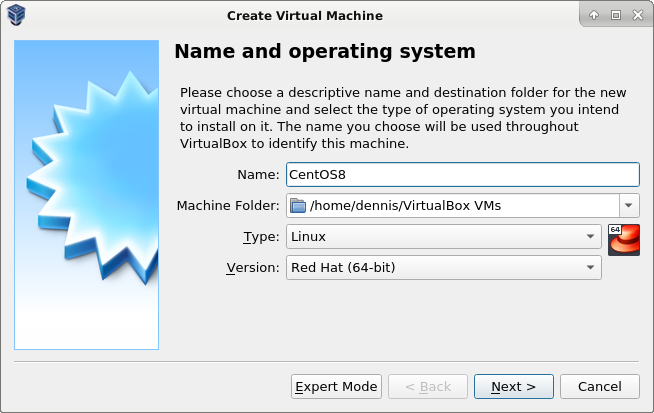
\includegraphics[width=0.99\linewidth]{linuxreader-img004.png}%
		}
		\end{minipage}
	\item Kies voor een 15 GB harddisk (VDI) die dynamisch mag groeien en 2 GB RAM.

	\item Als de machine aangemaakt is gaan we de netwerk settings wijzigen. We selecteren de machine en clicken op Properties. Bij Settings kiezen we voor Network.
	\item
		\begin{minipage}[t]{\linewidth}
		\raggedright
		\adjustbox{valign=t}{%
			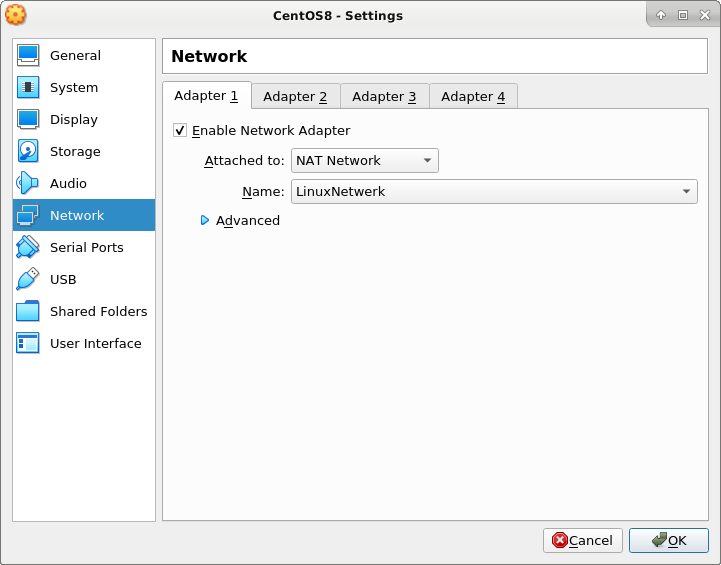
\includegraphics[width=0.99\linewidth]{linuxreader-img005.png}%
		}
		Wijzig bij Attached to: de setting naar NAT Network en selecteer vervolgens bij Name: het LinuxNewerk. Click op OK om de gemaakte wijzigingen op te slaan.
		\end{minipage}

\end{enumerate}
